\documentclass[a4paper, 12pt]{article}
\usepackage[pdftex, hidelinks]{hyperref}

\usepackage{bm}
\usepackage[T1]{fontenc}
\usepackage[utf8]{inputenc}
\usepackage{algorithmic}
\usepackage{algorithm}
\usepackage{amsfonts}
\usepackage{amssymb}
\usepackage{courier}
\usepackage{booktabs}
\usepackage{graphicx}
\usepackage{listings}
\usepackage{mathtools}
\usepackage{amssymb}
\lstset{basicstyle=\footnotesize\ttfamily,
breakatwhitespace = false,
breaklines = true,
keepspaces = true,
language = R,
showspaces = false,
showstringspaces = false,
belowcaptionskip = \bigskipamount,
framerule = 0.80pt,
frame = tb,
belowskip = \bigskipamount,
escapeinside={<@}{@>}}

\title{TDDE01 -- Machine Learning \\
Laboration Report 5}
\author{{Martin Estgren \texttt{<mares480>}} \\
{Linköping University (LiU), Sweden}}

\begin{document}
\pagenumbering{arabic}
    \maketitle % Generate.

    In this assignment we will use \textit{kernel methods} in order to determine the \textit{air temperature} for a given \textit{location}, \textit{time of day}, and \textit{date}. To realize this task we create three separate kernel methods \(k_{distance}(\hat{x}, x)\),\(k_{time}(\hat{x}, x)\),\(k_{date}(\hat{x}, x)\), each of which will be weighted by the respective weights \(w_{distance}, w_{time}, w_{date}\). The \(\hat{x}\) indicates a sampled data point and the \(x\) the given point we want to predict. The weights will be determined by reasoning about the relevance of each kernel.

    The kernel method is defined as the following function
    \begin{equation}
        k(\hat{x}, x) = k_{distance}(\hat{x}, x) + k_{time}(\hat{x}, x) + k_{date}(\hat{x}, x)
    \end{equation}
    and the respective kernel methods defined as:
    \begin{equation}
        k_{distance}(\hat{x}, x) = e^{-(\frac{haversine(\hat{x}, x)}{w_{disstance}})^2}
    \end{equation}
       \begin{equation}
        k_{time}(\hat{x}, x) = 
                \begin{cases}
        e^{-(\frac{\left |x - \hat{x} \right |}{w_{tim}})^2} & \text{ if } \left |x - \hat{x} \right | \le 12 \\ 
        e^{-(\frac{\left |x - (24- \hat{x}) \right |}{w_{tim}})^2} & \text{ if }  \left |x - \hat{x} \right | > 12 
        \end{cases}     
    \end{equation}

    \begin{equation}
        k_{time}(\hat{x}, x) = 
        \begin{cases}
        e^{-(\frac{\left |x - \hat{x}\right |}{w_{date}})^2} & \text{ if } \left |x - \hat{x}\right | \le 182 \\ 
        e^{-(\frac{\left |x - (365- \hat{x})\right |}{w_{date}})^2} & \text{ if }  \left |x - \hat{x}\right | > 182 
        \end{cases}     
    \end{equation}

    Below are the different kernel and Gaussian functions shown, as implemented in R.  The full code can be found in appendix 1.

    The Gaussian window function
    \lstinputlisting[firstline=23,lastline=25]{../share/script.r}
    
    The distance-kernel function \(k_{distance}(\hat{x}, x)\)
    \lstinputlisting[firstline=28,lastline=32]{../share/script.r}

    The time-kernel function \(k_{time}(\hat{x}, x)\)
    \lstinputlisting[firstline=45,lastline=51]{../share/script.r}

    The date-kernel \(k_{date}(\hat{x}, x)\)
    \lstinputlisting[firstline=35,lastline=42]{../share/script.r}
    
    We also need to modify the \textit{time} and \textit{date} features to make them compliant with our functions.
    \lstinputlisting[firstline=104,lastline=108]{../share/script.r}

    The above mentioned function are tied together in the garden keeper function:
    \lstinputlisting[firstline=54,lastline=101]{../share/script.r}
    Which also perform the temperature estimation by taking the mean of the kernel-values and their respective data points air temperature.

    \section{Result}

    Below are the result from the different kernel-methods and the result produced.
    
    \begin{figure}[H]
    \centering
    \caption{Distance plot (time of day) for the observations (Ordered by time of day) \label{fig:time}}
        \begin{minipage}[]{0.2\textwidth}
            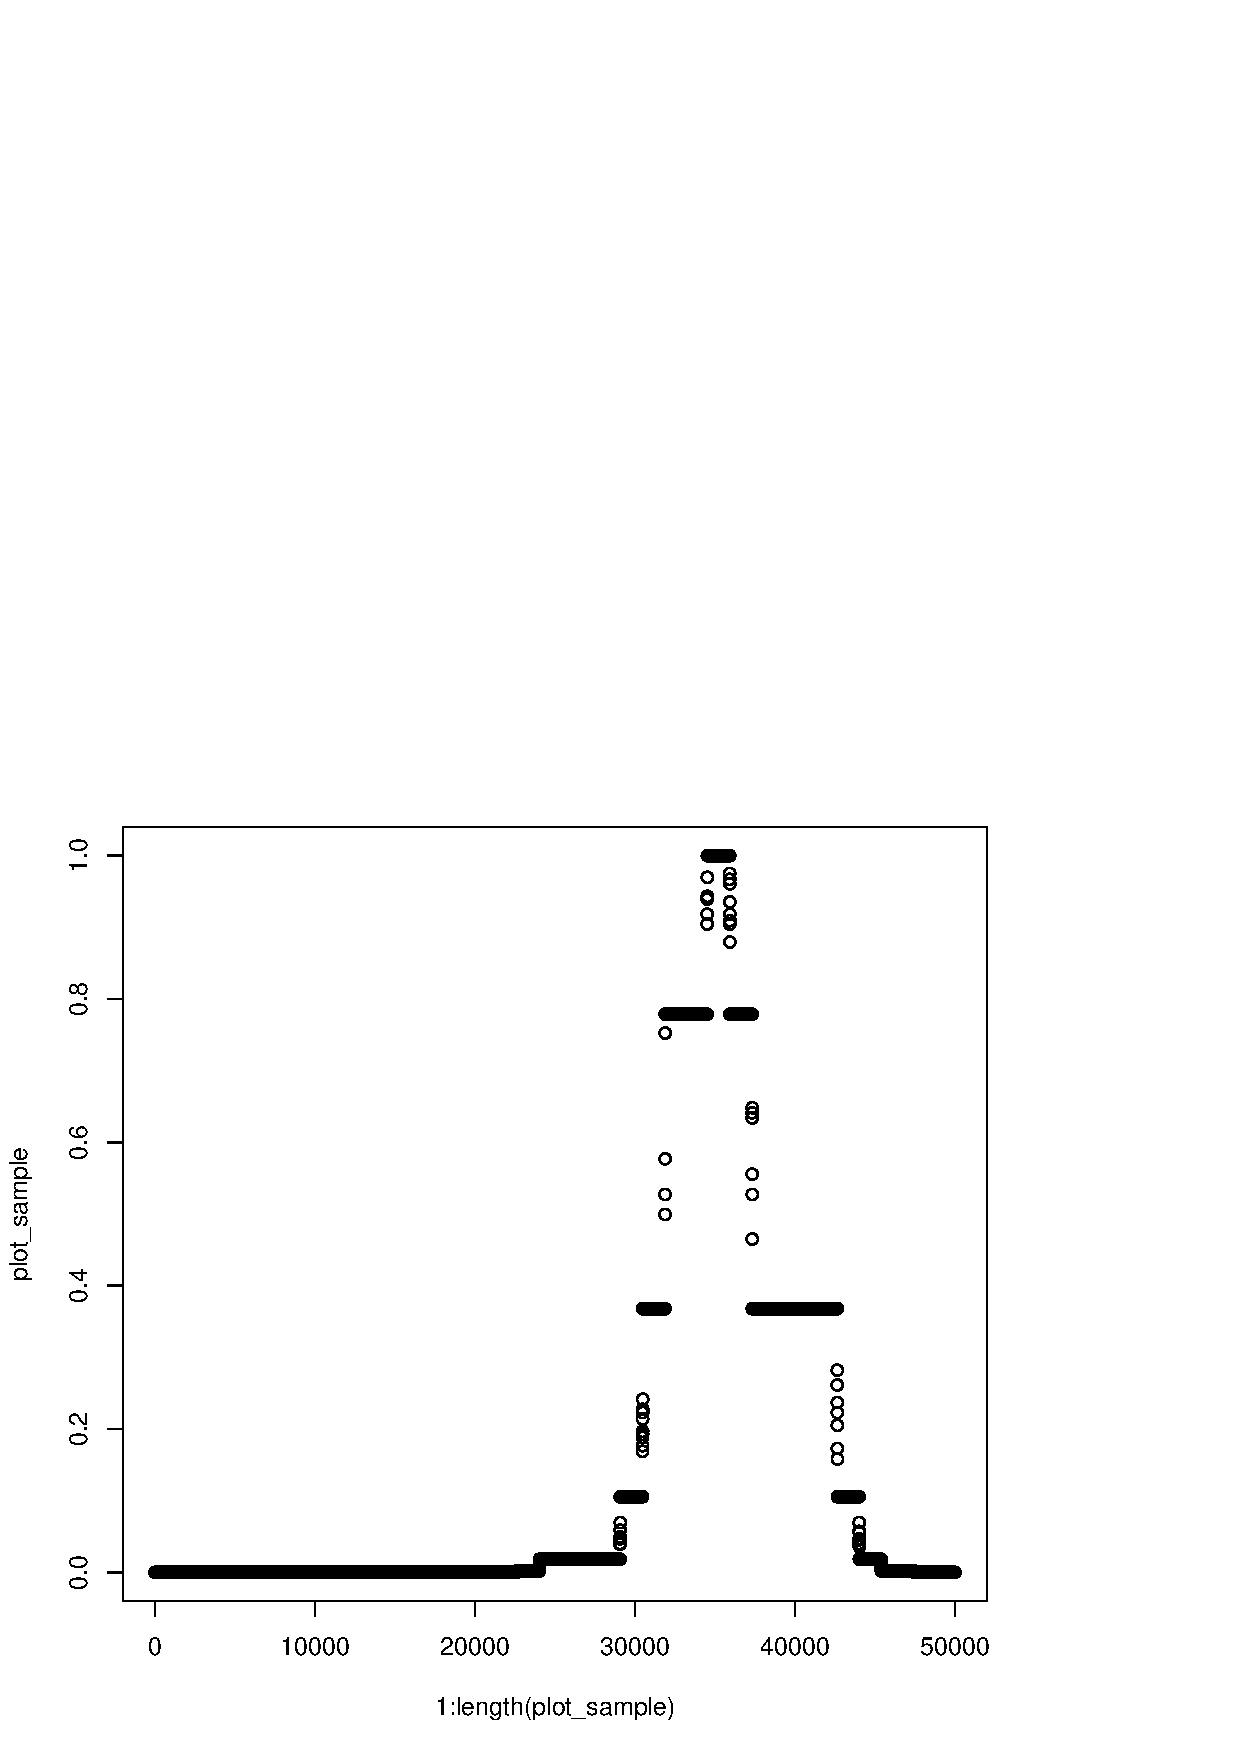
\includegraphics[width=\textwidth]{share/1_time.png}
        \end{minipage}
        \begin{minipage}[]{0.2\textwidth}
            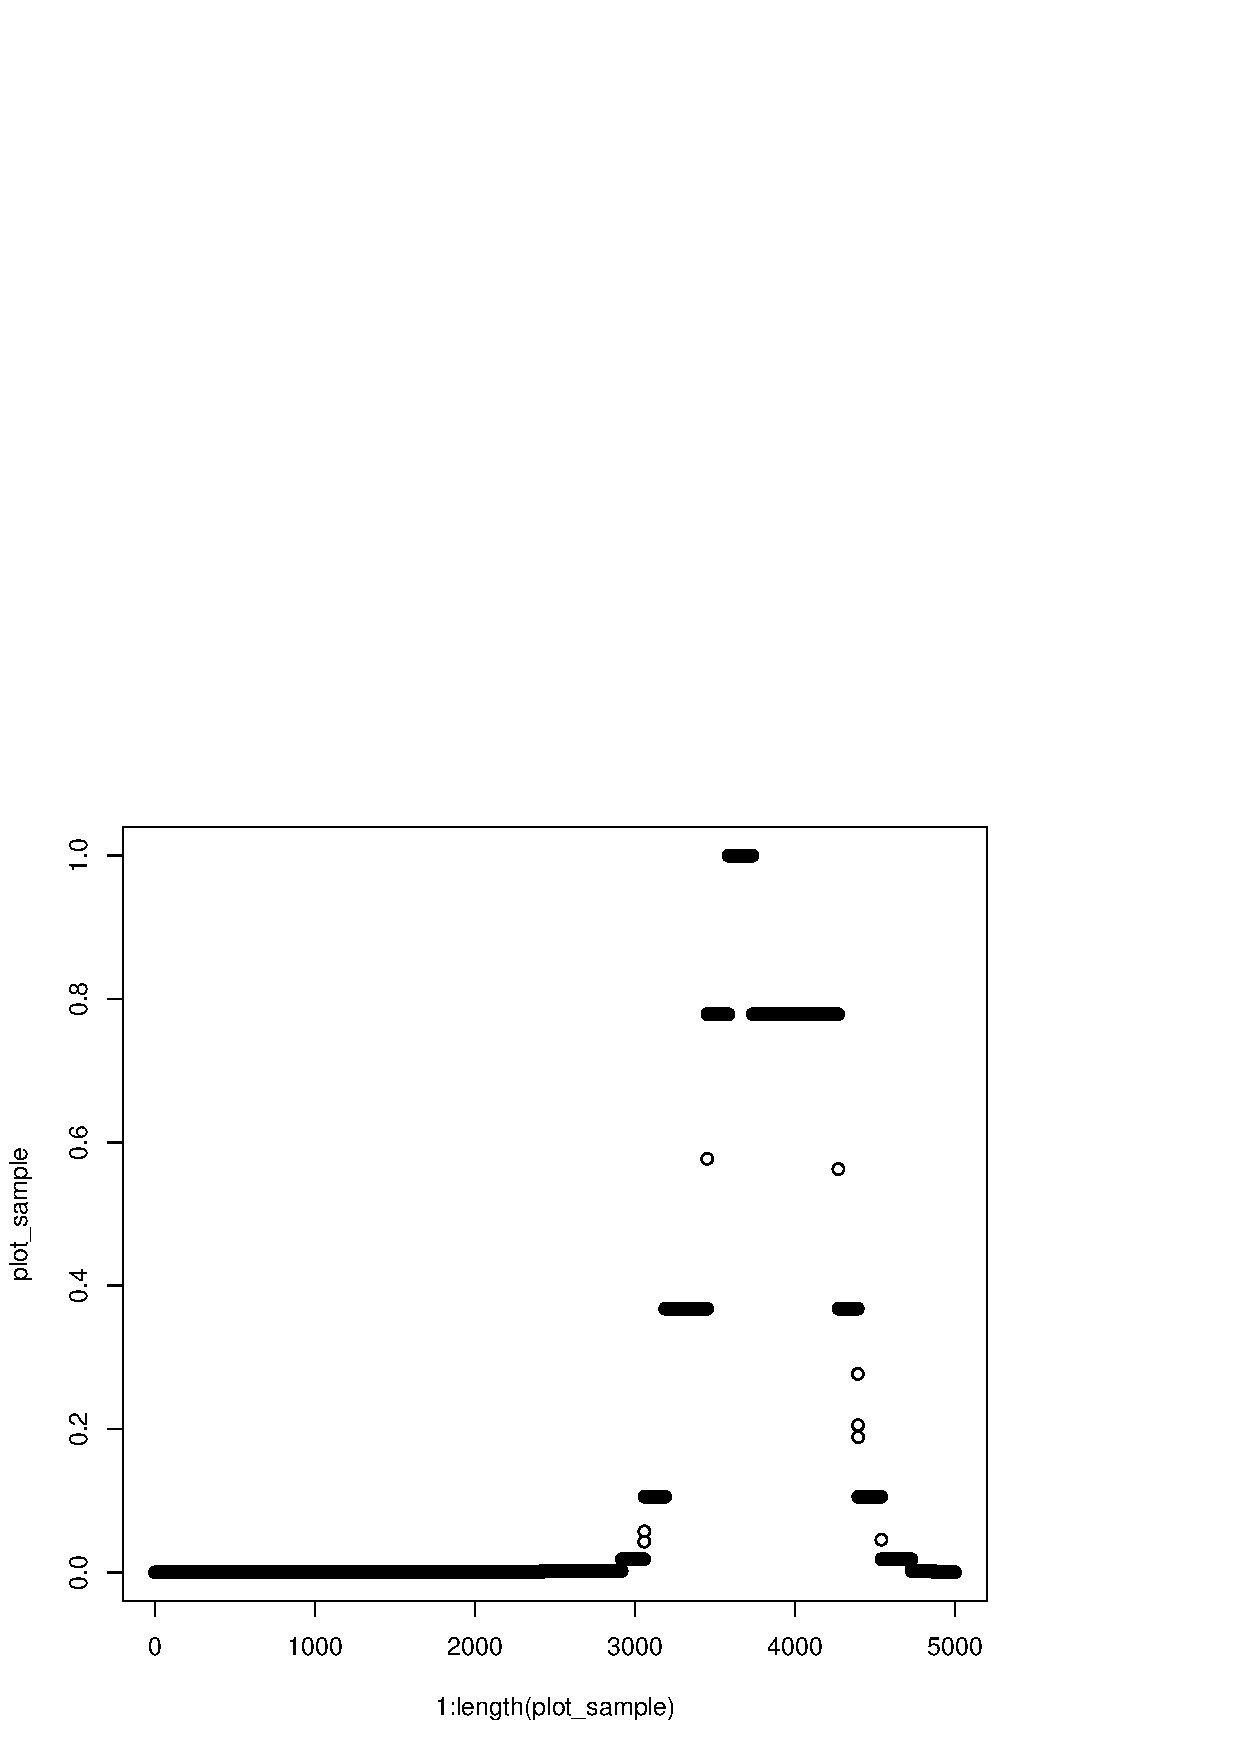
\includegraphics[width=\textwidth]{share/2_time.png}
        \end{minipage}
        \begin{minipage}[]{0.2\textwidth}
            \includegraphics[width=\textwidth]{share/3_time.png}
        \end{minipage}
        \begin{minipage}[]{0.2\textwidth}
            \includegraphics[width=\textwidth]{share/4_time.png}
        \end{minipage}
        \begin{minipage}[]{0.2\textwidth}
             \includegraphics[width=\textwidth]{share/5_time.png}
        \end{minipage}
        \begin{minipage}[]{0.2\textwidth}
            \includegraphics[width=\textwidth]{share/6_time.png}
        \end{minipage}
        \begin{minipage}[]{0.2\textwidth}
            \includegraphics[width=\textwidth]{share/7_time.png}
        \end{minipage}
        \begin{minipage}[]{0.2\textwidth}
             \includegraphics[width=\textwidth]{share/8_time.png}
        \end{minipage}
        \begin{minipage}[]{0.2\textwidth}
            \includegraphics[width=\textwidth]{share/9_time.png}
        \end{minipage}
        \begin{minipage}[]{0.2\textwidth}
            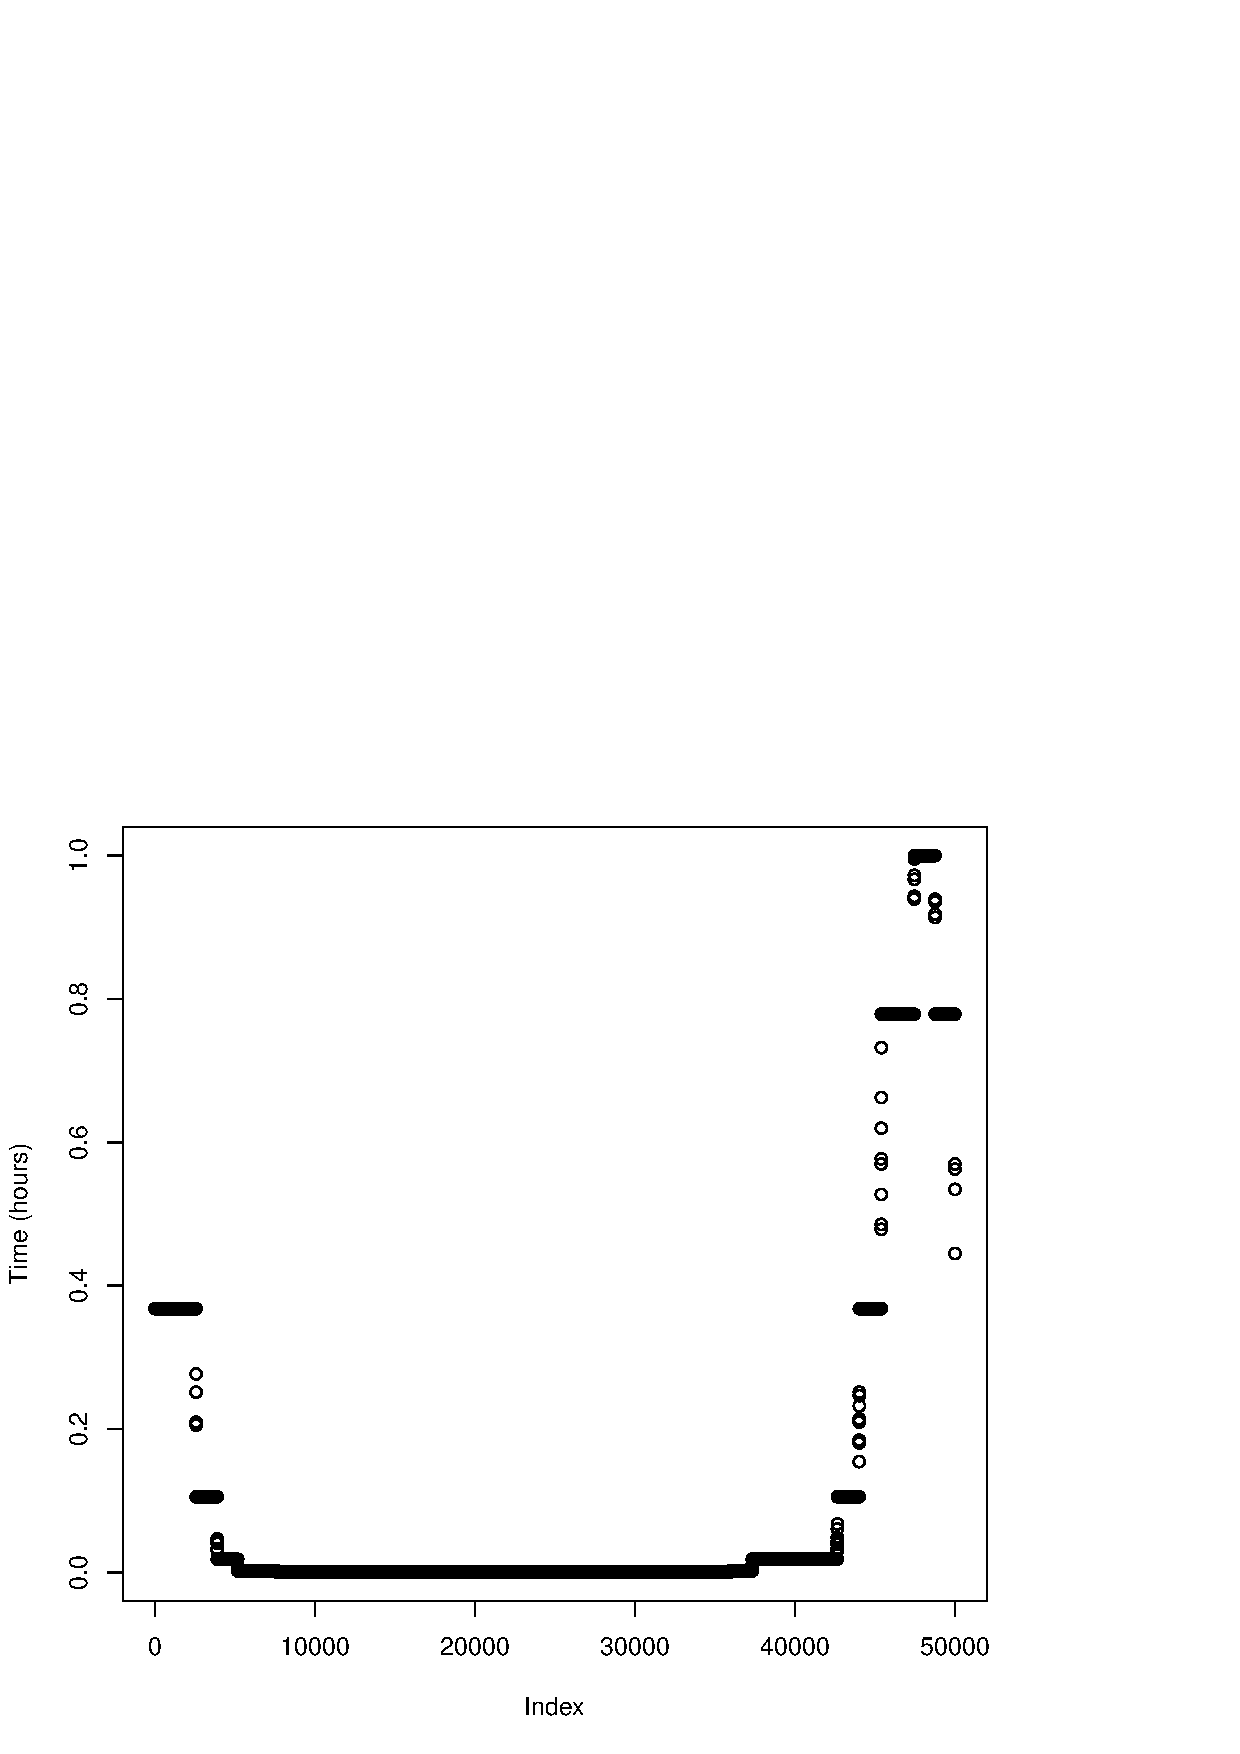
\includegraphics[width=\textwidth]{share/10_time.png}
        \end{minipage}
        \begin{minipage}[]{0.2\textwidth}
            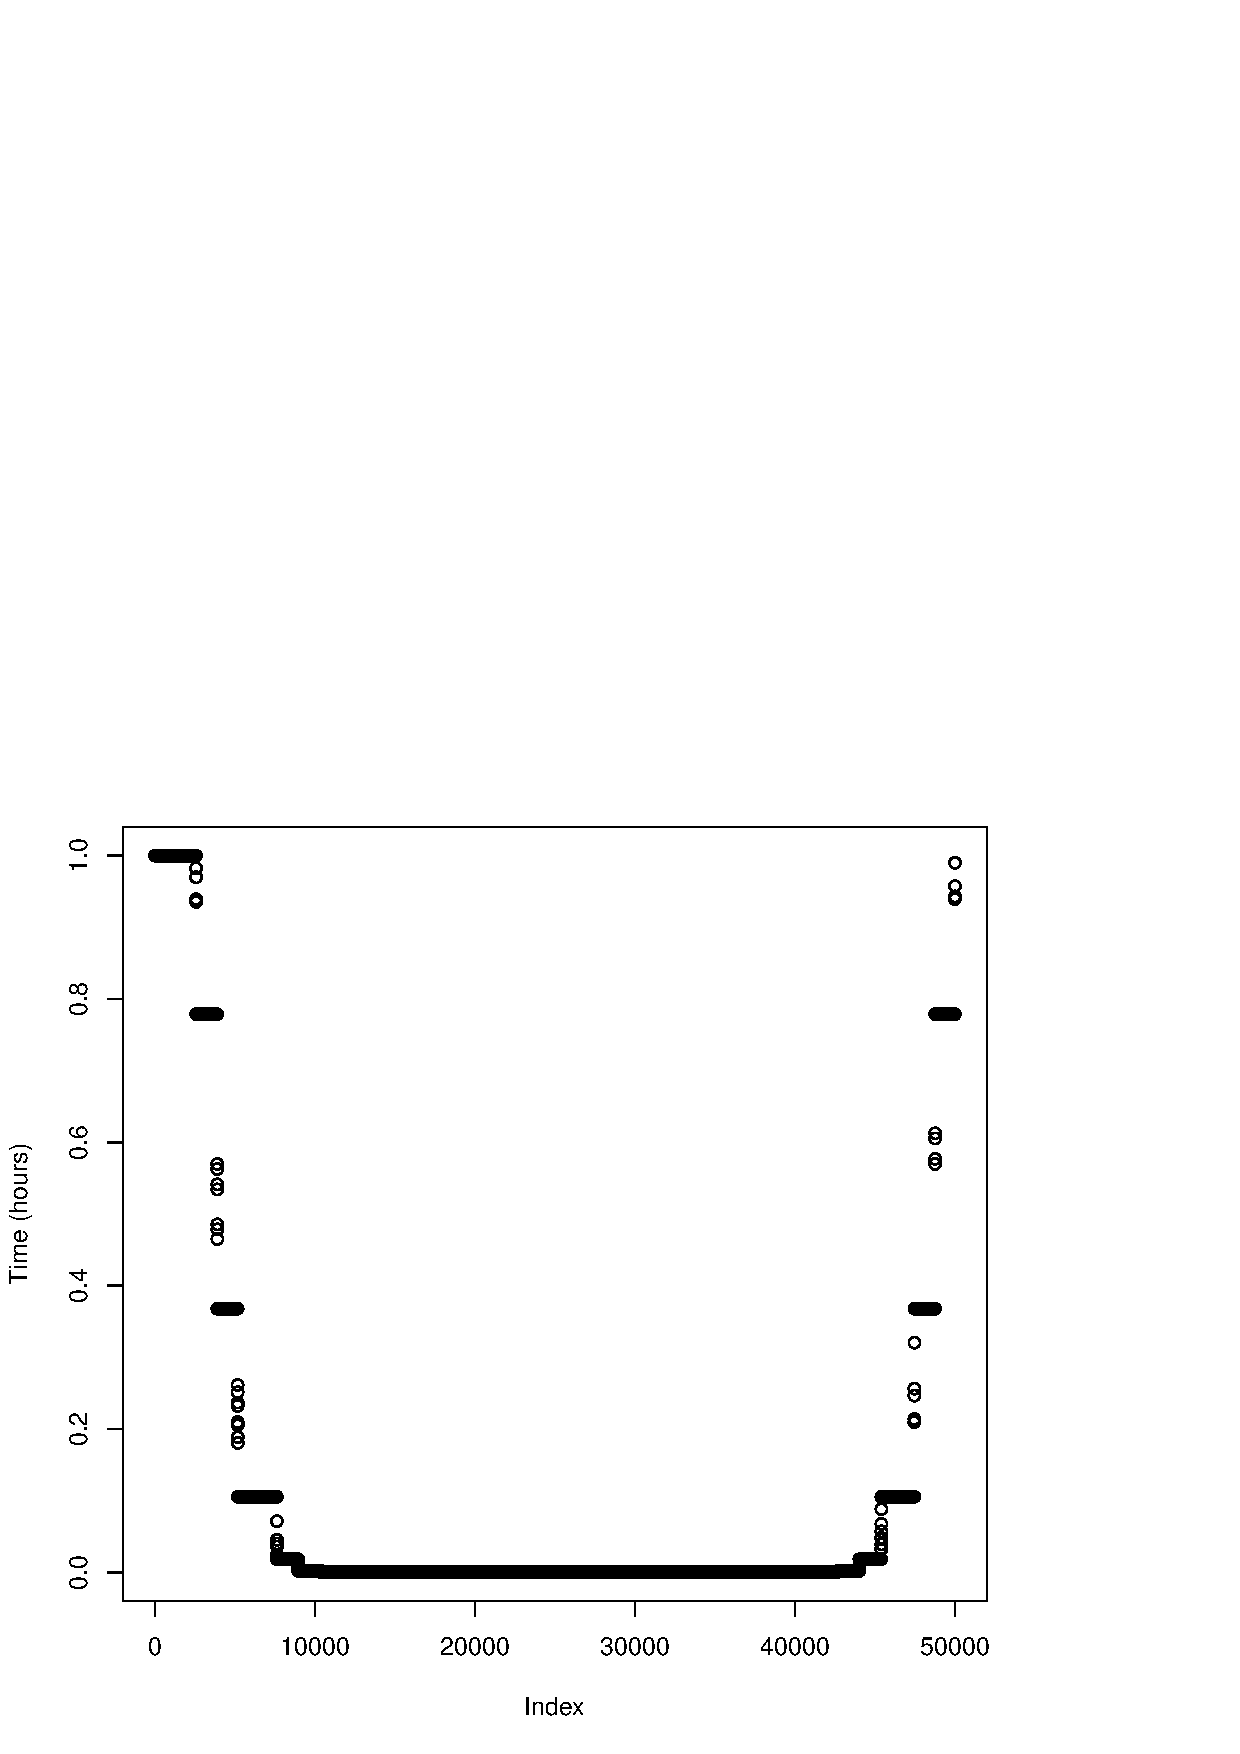
\includegraphics[width=\textwidth]{share/11_time.png}
        \end{minipage}
    \end{figure}

    We can clearly see a increase in kernel value the closer to the actual hour we observe. This would indicate how our choice for the kernel width of the time-kernel is reasonable.

    \begin{figure}[H]
    \centering
        \begin{minipage}[]{0.4\textwidth}
            \caption{Distance plot (day of year) for the observations (Ordered by month/day)\label{fig:day}}
            \includegraphics[width=\textwidth]{share/1_date.png}
        \end{minipage}
        \begin{minipage}[]{0.4\textwidth}
            \caption{Distance plot (day of year) for the observations (ordered by station)\label{fig:dist}}
            \includegraphics[width=\textwidth]{share/1_dist.png}
        \end{minipage}
    \end{figure}
    The figures above shows the distance of the date-kernel given the observation specified above. As with the \textit{time-kernel} we see an increase around the date of our observation, but much lower window size. he reasoning for this choice is that I believe the day of the year affects the result much greater than the time of day or location.
    The pattern is a bit harder to spot on the longitude/latitude figure because although there's a relation between station number and location they are not one and the same. We can still observe a increase in kernel value around the longitude and latitude of the observation.

    Below we have the plot of the observations.
    \begin{figure}[H]
    \centering
    \caption{Predicted temperature for the day 2013-04-12 in the interval 04:00-24:00 (ordered by hour)\label{fig:result}}
        \begin{minipage}[]{0.4\textwidth}
            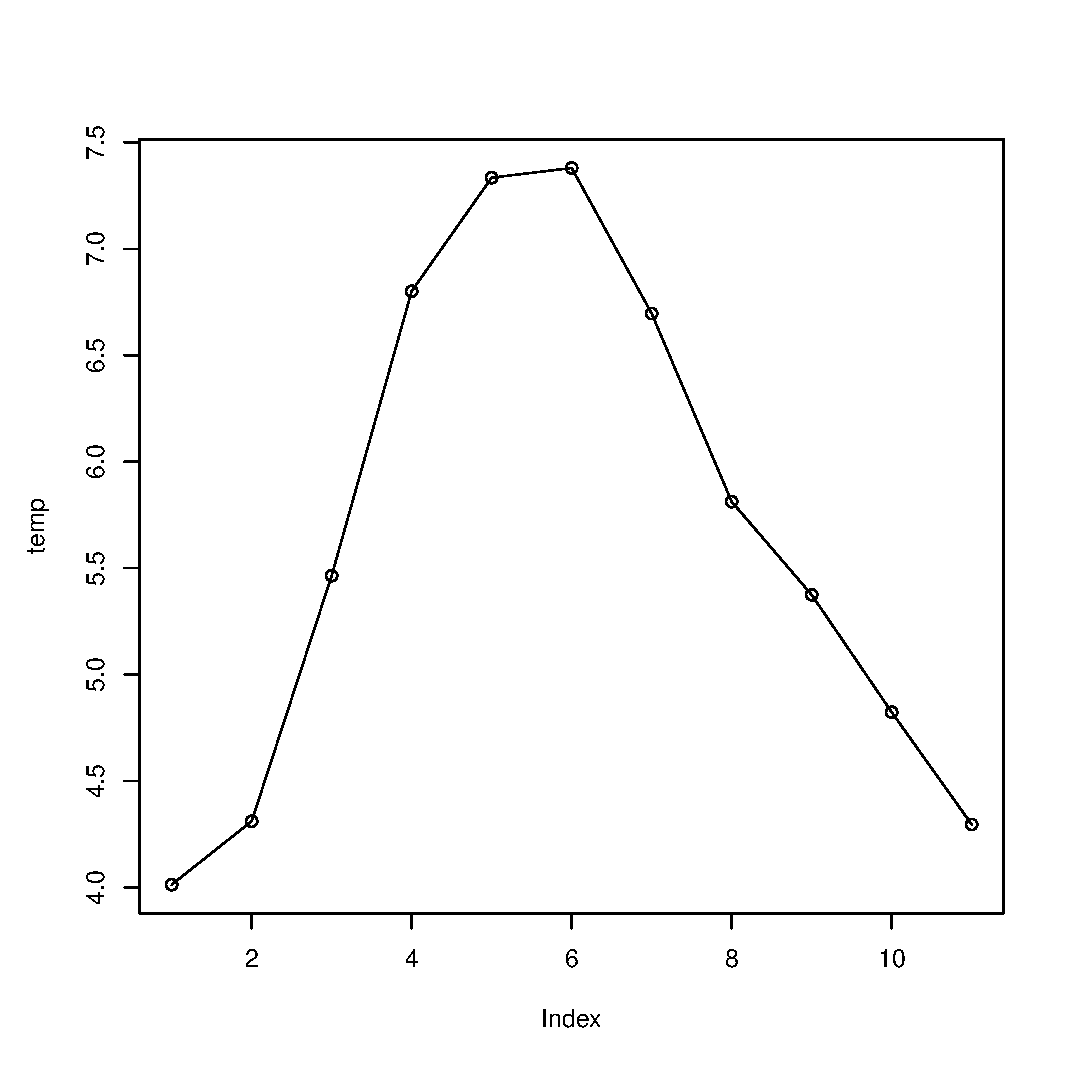
\includegraphics[width=\textwidth]{share/result.eps}
        \end{minipage}
    \end{figure}
    As expected we can observe how the temperature first increases, the decreases during the time of a typical day. The date would also place the temperature range in the same area as the result figure. This is more of a  coincident, the reason for which will be explained after the next figure. The \textit{weights} for each kernel was set to \(w_{distance} = 100000 \),\(w_{time} = 2 \), and \(w_{date} = 3\) respectively. The reason for this is that the geographic distance have a very large magnitude which first needs to be made manageable, otherwise all the distances no matter how close would result in the same kernel value. It was set to 100000 since that value allowed for most data points to contribute a little bit. 

    The time weight was set to 2 since we reasoned the time of day would be an significant factor and shouldn't therefore be reduced much. 

    The date-weight was set to 3 since, as with the time-weight, we reasoned that it would be an significant feature. Looking at the figure\ref{fig:day} and the result in \ref{fig:result} we may reason it could be raised a bit, perhaps closer to 10 if less precision would be needed.

    \begin{figure}[H]
    \centering
    \caption{Predicted temperature for the day 2013-07-12 in the interval 04:00-24:00 (ordered by hour)\label{fig:bad_result}}
        \begin{minipage}[]{0.4\textwidth}
            \includegraphics[width=\textwidth]{share/bad_result.eps}
        \end{minipage}
    \end{figure}
    In this figure we can observe the temperature for another day. This time in the middle of summer. The values doesn't differ much from the day in April. This could be explained by the fact that the kernel features are independent and therefore nonindependent targets hours/days/locations all year around. This will make all results gravitate towards the year-mean temperature which is around \(4.6^\circ\). Possible solutions could be to limit the influence of far-away data points by only picking the \(N\) best from each kernel. The result would be more precise but the number of distances to select would have to vary depending on the data set, adding additional complexity to an already complex model.

    \nocite{*} % No warnings.
    \bibliographystyle{alpha}
    \bibliography{report}
    \onecolumn \appendix
    \section*{Appendix}
    \lstinputlisting[caption={Script for Assignment},label={lst:script}]{../share/script.r}


    \end{document}
